\documentclass[twoside]{book}

% Packages required by doxygen
\usepackage{calc}
\usepackage{doxygen}
\usepackage{graphicx}
\usepackage[utf8]{inputenc}
\usepackage{makeidx}
\usepackage{multicol}
\usepackage{multirow}
\usepackage{textcomp}
\usepackage[table]{xcolor}

% Font selection
\usepackage[T1]{fontenc}
\usepackage{mathptmx}
\usepackage[scaled=.90]{helvet}
\usepackage{courier}
\usepackage{amssymb}
\usepackage{sectsty}
\renewcommand{\familydefault}{\sfdefault}
\allsectionsfont{%
  \fontseries{bc}\selectfont%
  \color{darkgray}%
}
\renewcommand{\DoxyLabelFont}{%
  \fontseries{bc}\selectfont%
  \color{darkgray}%
}

% Page & text layout
\usepackage{geometry}
\geometry{%
  a4paper,%
  top=2.5cm,%
  bottom=2.5cm,%
  left=2.5cm,%
  right=2.5cm%
}
\tolerance=750
\hfuzz=15pt
\hbadness=750
\setlength{\emergencystretch}{15pt}
\setlength{\parindent}{0cm}
\setlength{\parskip}{0.2cm}
\makeatletter
\renewcommand{\paragraph}{%
  \@startsection{paragraph}{4}{0ex}{-1.0ex}{1.0ex}{%
    \normalfont\normalsize\bfseries\SS@parafont%
  }%
}
\renewcommand{\subparagraph}{%
  \@startsection{subparagraph}{5}{0ex}{-1.0ex}{1.0ex}{%
    \normalfont\normalsize\bfseries\SS@subparafont%
  }%
}
\makeatother

% Headers & footers
\usepackage{fancyhdr}
\pagestyle{fancyplain}
\fancyhead[LE]{\fancyplain{}{\bfseries\thepage}}
\fancyhead[CE]{\fancyplain{}{}}
\fancyhead[RE]{\fancyplain{}{\bfseries\leftmark}}
\fancyhead[LO]{\fancyplain{}{\bfseries\rightmark}}
\fancyhead[CO]{\fancyplain{}{}}
\fancyhead[RO]{\fancyplain{}{\bfseries\thepage}}
\fancyfoot[LE]{\fancyplain{}{}}
\fancyfoot[CE]{\fancyplain{}{}}
\fancyfoot[RE]{\fancyplain{}{\bfseries\scriptsize Generated on Fri Apr 13 2018 14\-:53\-:53 for My Project by Doxygen }}
\fancyfoot[LO]{\fancyplain{}{\bfseries\scriptsize Generated on Fri Apr 13 2018 14\-:53\-:53 for My Project by Doxygen }}
\fancyfoot[CO]{\fancyplain{}{}}
\fancyfoot[RO]{\fancyplain{}{}}
\renewcommand{\footrulewidth}{0.4pt}
\renewcommand{\chaptermark}[1]{%
  \markboth{#1}{}%
}
\renewcommand{\sectionmark}[1]{%
  \markright{\thesection\ #1}%
}

% Indices & bibliography
\usepackage{natbib}
\usepackage[titles]{tocloft}
\setcounter{tocdepth}{3}
\setcounter{secnumdepth}{5}
\makeindex

% Hyperlinks (required, but should be loaded last)
\usepackage{ifpdf}
\ifpdf
  \usepackage[pdftex,pagebackref=true]{hyperref}
\else
  \usepackage[ps2pdf,pagebackref=true]{hyperref}
\fi
\hypersetup{%
  colorlinks=true,%
  linkcolor=blue,%
  citecolor=blue,%
  unicode%
}

% Custom commands
\newcommand{\clearemptydoublepage}{%
  \newpage{\pagestyle{empty}\cleardoublepage}%
}


%===== C O N T E N T S =====

\begin{document}

% Titlepage & ToC
\hypersetup{pageanchor=false}
\pagenumbering{roman}
\begin{titlepage}
\vspace*{7cm}
\begin{center}%
{\Large My Project }\\
\vspace*{1cm}
{\large Generated by Doxygen 1.8.6}\\
\vspace*{0.5cm}
{\small Fri Apr 13 2018 14:53:53}\\
\end{center}
\end{titlepage}
\clearemptydoublepage
\tableofcontents
\clearemptydoublepage
\pagenumbering{arabic}
\hypersetup{pageanchor=true}

%--- Begin generated contents ---
\chapter{Namespace Index}
\section{Namespace List}
Here is a list of all namespaces with brief descriptions\-:\begin{DoxyCompactList}
\item\contentsline{section}{\hyperlink{namespacePRNT}{P\-R\-N\-T} }{\pageref{namespacePRNT}}{}
\end{DoxyCompactList}

\chapter{Class Index}
\section{Class List}
Here are the classes, structs, unions and interfaces with brief descriptions\-:\begin{DoxyCompactList}
\item\contentsline{section}{\hyperlink{structcout__redirect}{cout\-\_\-redirect} }{\pageref{structcout__redirect}}{}
\item\contentsline{section}{\hyperlink{structhelper}{helper} }{\pageref{structhelper}}{}
\item\contentsline{section}{\hyperlink{classPRNT_1_1print__ip}{P\-R\-N\-T\-::print\-\_\-ip$<$ T, bool, bool $>$} }{\pageref{classPRNT_1_1print__ip}}{}
\item\contentsline{section}{\hyperlink{classPRNT_1_1print__ip_3_01std_1_1string_00_01false_00_01true_01_4}{P\-R\-N\-T\-::print\-\_\-ip$<$ std\-::string, false, true $>$} }{\pageref{classPRNT_1_1print__ip_3_01std_1_1string_00_01false_00_01true_01_4}}{}
\item\contentsline{section}{\hyperlink{classPRNT_1_1print__ip_3_01T_00_01false_00_01true_01_4}{P\-R\-N\-T\-::print\-\_\-ip$<$ T, false, true $>$} }{\pageref{classPRNT_1_1print__ip_3_01T_00_01false_00_01true_01_4}}{}
\item\contentsline{section}{\hyperlink{classPRNT_1_1print__ip_3_01T_00_01true_00_01false_01_4}{P\-R\-N\-T\-::print\-\_\-ip$<$ T, true, false $>$} }{\pageref{classPRNT_1_1print__ip_3_01T_00_01true_00_01false_01_4}}{}
\end{DoxyCompactList}

\chapter{File Index}
\section{File List}
Here is a list of all files with brief descriptions\-:\begin{DoxyCompactList}
\item\contentsline{section}{\hyperlink{main_8cpp}{main.\-cpp} }{\pageref{main_8cpp}}{}
\item\contentsline{section}{\hyperlink{print__ip_8h}{print\-\_\-ip.\-h} }{\pageref{print__ip_8h}}{}
\item\contentsline{section}{\hyperlink{tests_8cpp}{tests.\-cpp} }{\pageref{tests_8cpp}}{}
\item\contentsline{section}{\hyperlink{version_8h}{version.\-h} }{\pageref{version_8h}}{}
\end{DoxyCompactList}

\chapter{Namespace Documentation}
\hypertarget{namespacePRNT}{\section{P\-R\-N\-T Namespace Reference}
\label{namespacePRNT}\index{P\-R\-N\-T@{P\-R\-N\-T}}
}
\subsection*{Classes}
\begin{DoxyCompactItemize}
\item 
class \hyperlink{classPRNT_1_1print__ip}{print\-\_\-ip}
\item 
class \hyperlink{classPRNT_1_1print__ip_3_01std_1_1string_00_01false_00_01true_01_4}{print\-\_\-ip$<$ std\-::string, false, true $>$}
\item 
class \hyperlink{classPRNT_1_1print__ip_3_01T_00_01false_00_01true_01_4}{print\-\_\-ip$<$ T, false, true $>$}
\item 
class \hyperlink{classPRNT_1_1print__ip_3_01T_00_01true_00_01false_01_4}{print\-\_\-ip$<$ T, true, false $>$}
\end{DoxyCompactItemize}
\subsection*{Functions}
\begin{DoxyCompactItemize}
\item 
{\footnotesize template$<$size\-\_\-t I = 0, typename... Tp$>$ }\\std\-::enable\-\_\-if$<$ I==sizeof...(Tp), \\*
void $>$\-::type \hyperlink{namespacePRNT_a034dd46fbd618b4c1e2d8b4612b676ef}{print} (const std\-::tuple$<$ Tp...$>$ \&t)
\end{DoxyCompactItemize}


\subsection{Function Documentation}
\hypertarget{namespacePRNT_a034dd46fbd618b4c1e2d8b4612b676ef}{\index{P\-R\-N\-T@{P\-R\-N\-T}!print@{print}}
\index{print@{print}!PRNT@{P\-R\-N\-T}}
\subsubsection[{print}]{\setlength{\rightskip}{0pt plus 5cm}template$<$size\-\_\-t I = 0, typename... Tp$>$ std\-::enable\-\_\-if$<$I == sizeof...(Tp), void$>$\-::type P\-R\-N\-T\-::print (
\begin{DoxyParamCaption}
\item[{const std\-::tuple$<$ Tp...$>$ \&}]{t}
\end{DoxyParamCaption}
)}}\label{namespacePRNT_a034dd46fbd618b4c1e2d8b4612b676ef}

\chapter{Class Documentation}
\hypertarget{structcout__redirect}{\section{cout\-\_\-redirect Struct Reference}
\label{structcout__redirect}\index{cout\-\_\-redirect@{cout\-\_\-redirect}}
}
\subsection*{Public Member Functions}
\begin{DoxyCompactItemize}
\item 
\hyperlink{structcout__redirect_a1ce2b56b3bf54f8bbd2709828e517946}{cout\-\_\-redirect} (std\-::streambuf $\ast$new\-\_\-buffer)
\item 
\hyperlink{structcout__redirect_a6f5fcbfd32ccdc91684fb4c91d170001}{$\sim$cout\-\_\-redirect} ()
\end{DoxyCompactItemize}


\subsection{Constructor \& Destructor Documentation}
\hypertarget{structcout__redirect_a1ce2b56b3bf54f8bbd2709828e517946}{\index{cout\-\_\-redirect@{cout\-\_\-redirect}!cout\-\_\-redirect@{cout\-\_\-redirect}}
\index{cout\-\_\-redirect@{cout\-\_\-redirect}!cout_redirect@{cout\-\_\-redirect}}
\subsubsection[{cout\-\_\-redirect}]{\setlength{\rightskip}{0pt plus 5cm}cout\-\_\-redirect\-::cout\-\_\-redirect (
\begin{DoxyParamCaption}
\item[{std\-::streambuf $\ast$}]{new\-\_\-buffer}
\end{DoxyParamCaption}
)\hspace{0.3cm}{\ttfamily [inline]}}}\label{structcout__redirect_a1ce2b56b3bf54f8bbd2709828e517946}
\hypertarget{structcout__redirect_a6f5fcbfd32ccdc91684fb4c91d170001}{\index{cout\-\_\-redirect@{cout\-\_\-redirect}!$\sim$cout\-\_\-redirect@{$\sim$cout\-\_\-redirect}}
\index{$\sim$cout\-\_\-redirect@{$\sim$cout\-\_\-redirect}!cout_redirect@{cout\-\_\-redirect}}
\subsubsection[{$\sim$cout\-\_\-redirect}]{\setlength{\rightskip}{0pt plus 5cm}cout\-\_\-redirect\-::$\sim$cout\-\_\-redirect (
\begin{DoxyParamCaption}
{}
\end{DoxyParamCaption}
)\hspace{0.3cm}{\ttfamily [inline]}}}\label{structcout__redirect_a6f5fcbfd32ccdc91684fb4c91d170001}


The documentation for this struct was generated from the following file\-:\begin{DoxyCompactItemize}
\item 
\hyperlink{tests_8cpp}{tests.\-cpp}\end{DoxyCompactItemize}

\hypertarget{structhelper}{\section{helper Struct Reference}
\label{structhelper}\index{helper@{helper}}
}
\subsection*{Public Member Functions}
\begin{DoxyCompactItemize}
\item 
{\footnotesize template$<$typename T $>$ }\\void \hyperlink{structhelper_a24d8e8de4ff4d4b037b28ce1a079c682}{operator()} (T \&t) const 
\end{DoxyCompactItemize}


\subsection{Member Function Documentation}
\hypertarget{structhelper_a24d8e8de4ff4d4b037b28ce1a079c682}{\index{helper@{helper}!operator()@{operator()}}
\index{operator()@{operator()}!helper@{helper}}
\subsubsection[{operator()}]{\setlength{\rightskip}{0pt plus 5cm}template$<$typename T $>$ void helper\-::operator() (
\begin{DoxyParamCaption}
\item[{T \&}]{t}
\end{DoxyParamCaption}
) const\hspace{0.3cm}{\ttfamily [inline]}}}\label{structhelper_a24d8e8de4ff4d4b037b28ce1a079c682}


The documentation for this struct was generated from the following file\-:\begin{DoxyCompactItemize}
\item 
\hyperlink{tests_8cpp}{tests.\-cpp}\end{DoxyCompactItemize}

\hypertarget{classPRNT_1_1print__ip}{\section{P\-R\-N\-T\-:\-:print\-\_\-ip$<$ T, bool, bool $>$ Class Template Reference}
\label{classPRNT_1_1print__ip}\index{P\-R\-N\-T\-::print\-\_\-ip$<$ T, bool, bool $>$@{P\-R\-N\-T\-::print\-\_\-ip$<$ T, bool, bool $>$}}
}


{\ttfamily \#include $<$print\-\_\-ip.\-h$>$}



The documentation for this class was generated from the following file\-:\begin{DoxyCompactItemize}
\item 
\hyperlink{print__ip_8h}{print\-\_\-ip.\-h}\end{DoxyCompactItemize}

\hypertarget{classPRNT_1_1print__ip_3_01std_1_1string_00_01false_00_01true_01_4}{\section{P\-R\-N\-T\-:\-:print\-\_\-ip$<$ std\-:\-:string, false, true $>$ Class Template Reference}
\label{classPRNT_1_1print__ip_3_01std_1_1string_00_01false_00_01true_01_4}\index{P\-R\-N\-T\-::print\-\_\-ip$<$ std\-::string, false, true $>$@{P\-R\-N\-T\-::print\-\_\-ip$<$ std\-::string, false, true $>$}}
}


{\ttfamily \#include $<$print\-\_\-ip.\-h$>$}

\subsection*{Static Public Member Functions}
\begin{DoxyCompactItemize}
\item 
static void \hyperlink{classPRNT_1_1print__ip_3_01std_1_1string_00_01false_00_01true_01_4_aca9194155b0e4a63e6a938ab5098cc55}{print\-\_\-pr} (const std\-::string \&str)
\end{DoxyCompactItemize}


\subsection{Member Function Documentation}
\hypertarget{classPRNT_1_1print__ip_3_01std_1_1string_00_01false_00_01true_01_4_aca9194155b0e4a63e6a938ab5098cc55}{\index{P\-R\-N\-T\-::print\-\_\-ip$<$ std\-::string, false, true $>$@{P\-R\-N\-T\-::print\-\_\-ip$<$ std\-::string, false, true $>$}!print\-\_\-pr@{print\-\_\-pr}}
\index{print\-\_\-pr@{print\-\_\-pr}!PRNT::print_ip< std::string, false, true >@{P\-R\-N\-T\-::print\-\_\-ip$<$ std\-::string, false, true $>$}}
\subsubsection[{print\-\_\-pr}]{\setlength{\rightskip}{0pt plus 5cm}static void {\bf P\-R\-N\-T\-::print\-\_\-ip}$<$ std\-::string, false, true $>$\-::print\-\_\-pr (
\begin{DoxyParamCaption}
\item[{const std\-::string \&}]{str}
\end{DoxyParamCaption}
)\hspace{0.3cm}{\ttfamily [inline]}, {\ttfamily [static]}}}\label{classPRNT_1_1print__ip_3_01std_1_1string_00_01false_00_01true_01_4_aca9194155b0e4a63e6a938ab5098cc55}


The documentation for this class was generated from the following file\-:\begin{DoxyCompactItemize}
\item 
\hyperlink{print__ip_8h}{print\-\_\-ip.\-h}\end{DoxyCompactItemize}

\hypertarget{classPRNT_1_1print__ip_3_01T_00_01false_00_01true_01_4}{\section{P\-R\-N\-T\-:\-:print\-\_\-ip$<$ T, false, true $>$ Class Template Reference}
\label{classPRNT_1_1print__ip_3_01T_00_01false_00_01true_01_4}\index{P\-R\-N\-T\-::print\-\_\-ip$<$ T, false, true $>$@{P\-R\-N\-T\-::print\-\_\-ip$<$ T, false, true $>$}}
}


{\ttfamily \#include $<$print\-\_\-ip.\-h$>$}

\subsection*{Static Public Member Functions}
\begin{DoxyCompactItemize}
\item 
static void \hyperlink{classPRNT_1_1print__ip_3_01T_00_01false_00_01true_01_4_aaa0d9a0911fb466940acc219c9bc0736}{print\-\_\-pr} (const T \&vec)
\end{DoxyCompactItemize}


\subsection{Member Function Documentation}
\hypertarget{classPRNT_1_1print__ip_3_01T_00_01false_00_01true_01_4_aaa0d9a0911fb466940acc219c9bc0736}{\index{P\-R\-N\-T\-::print\-\_\-ip$<$ T, false, true $>$@{P\-R\-N\-T\-::print\-\_\-ip$<$ T, false, true $>$}!print\-\_\-pr@{print\-\_\-pr}}
\index{print\-\_\-pr@{print\-\_\-pr}!PRNT::print_ip< T, false, true >@{P\-R\-N\-T\-::print\-\_\-ip$<$ T, false, true $>$}}
\subsubsection[{print\-\_\-pr}]{\setlength{\rightskip}{0pt plus 5cm}template$<$typename T $>$ static void {\bf P\-R\-N\-T\-::print\-\_\-ip}$<$ T, false, true $>$\-::print\-\_\-pr (
\begin{DoxyParamCaption}
\item[{const T \&}]{vec}
\end{DoxyParamCaption}
)\hspace{0.3cm}{\ttfamily [inline]}, {\ttfamily [static]}}}\label{classPRNT_1_1print__ip_3_01T_00_01false_00_01true_01_4_aaa0d9a0911fb466940acc219c9bc0736}


The documentation for this class was generated from the following file\-:\begin{DoxyCompactItemize}
\item 
\hyperlink{print__ip_8h}{print\-\_\-ip.\-h}\end{DoxyCompactItemize}

\hypertarget{classPRNT_1_1print__ip_3_01T_00_01true_00_01false_01_4}{\section{P\-R\-N\-T\-:\-:print\-\_\-ip$<$ T, true, false $>$ Class Template Reference}
\label{classPRNT_1_1print__ip_3_01T_00_01true_00_01false_01_4}\index{P\-R\-N\-T\-::print\-\_\-ip$<$ T, true, false $>$@{P\-R\-N\-T\-::print\-\_\-ip$<$ T, true, false $>$}}
}


{\ttfamily \#include $<$print\-\_\-ip.\-h$>$}

\subsection*{Static Public Member Functions}
\begin{DoxyCompactItemize}
\item 
static void \hyperlink{classPRNT_1_1print__ip_3_01T_00_01true_00_01false_01_4_a5961e8e9bbc8b7202bb551d6cbb1b746}{print\-\_\-pr} (const T \&t)
\end{DoxyCompactItemize}


\subsection{Member Function Documentation}
\hypertarget{classPRNT_1_1print__ip_3_01T_00_01true_00_01false_01_4_a5961e8e9bbc8b7202bb551d6cbb1b746}{\index{P\-R\-N\-T\-::print\-\_\-ip$<$ T, true, false $>$@{P\-R\-N\-T\-::print\-\_\-ip$<$ T, true, false $>$}!print\-\_\-pr@{print\-\_\-pr}}
\index{print\-\_\-pr@{print\-\_\-pr}!PRNT::print_ip< T, true, false >@{P\-R\-N\-T\-::print\-\_\-ip$<$ T, true, false $>$}}
\subsubsection[{print\-\_\-pr}]{\setlength{\rightskip}{0pt plus 5cm}template$<$typename T $>$ static void {\bf P\-R\-N\-T\-::print\-\_\-ip}$<$ T, true, false $>$\-::print\-\_\-pr (
\begin{DoxyParamCaption}
\item[{const T \&}]{t}
\end{DoxyParamCaption}
)\hspace{0.3cm}{\ttfamily [inline]}, {\ttfamily [static]}}}\label{classPRNT_1_1print__ip_3_01T_00_01true_00_01false_01_4_a5961e8e9bbc8b7202bb551d6cbb1b746}


The documentation for this class was generated from the following file\-:\begin{DoxyCompactItemize}
\item 
\hyperlink{print__ip_8h}{print\-\_\-ip.\-h}\end{DoxyCompactItemize}

\chapter{File Documentation}
\hypertarget{main_8cpp}{\section{main.\-cpp File Reference}
\label{main_8cpp}\index{main.\-cpp@{main.\-cpp}}
}
{\ttfamily \#include $<$iostream$>$}\\*
{\ttfamily \#include $<$string$>$}\\*
{\ttfamily \#include $<$vector$>$}\\*
{\ttfamily \#include \char`\"{}print\-\_\-ip.\-h\char`\"{}}\\*
Include dependency graph for main.\-cpp\-:
\nopagebreak
\begin{figure}[H]
\begin{center}
\leavevmode
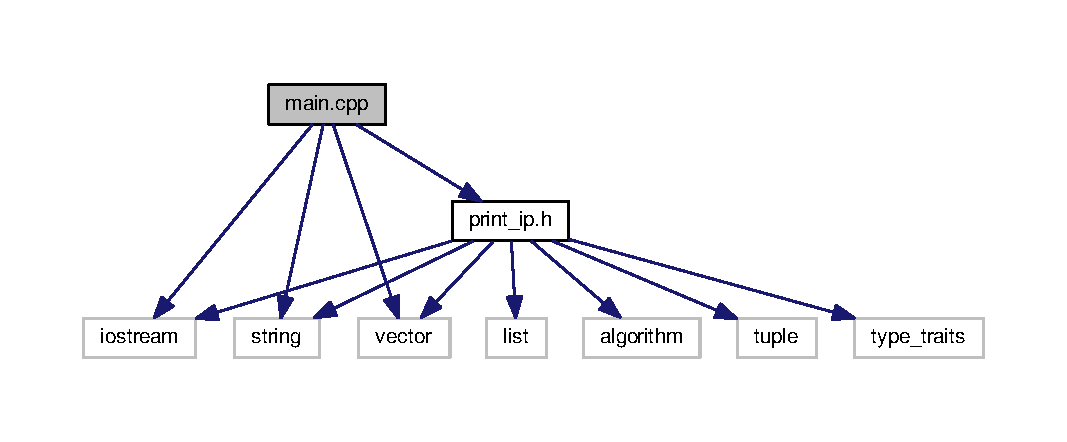
\includegraphics[width=350pt]{main_8cpp__incl}
\end{center}
\end{figure}
\subsection*{Functions}
\begin{DoxyCompactItemize}
\item 
int \hyperlink{main_8cpp_ae66f6b31b5ad750f1fe042a706a4e3d4}{main} ()
\end{DoxyCompactItemize}


\subsection{Function Documentation}
\hypertarget{main_8cpp_ae66f6b31b5ad750f1fe042a706a4e3d4}{\index{main.\-cpp@{main.\-cpp}!main@{main}}
\index{main@{main}!main.cpp@{main.\-cpp}}
\subsubsection[{main}]{\setlength{\rightskip}{0pt plus 5cm}int main (
\begin{DoxyParamCaption}
{}
\end{DoxyParamCaption}
)}}\label{main_8cpp_ae66f6b31b5ad750f1fe042a706a4e3d4}

\hypertarget{print__ip_8h}{\section{print\-\_\-ip.\-h File Reference}
\label{print__ip_8h}\index{print\-\_\-ip.\-h@{print\-\_\-ip.\-h}}
}
{\ttfamily \#include $<$string$>$}\\*
{\ttfamily \#include $<$type\-\_\-traits$>$}\\*
{\ttfamily \#include $<$vector$>$}\\*
{\ttfamily \#include $<$list$>$}\\*
{\ttfamily \#include $<$algorithm$>$}\\*
{\ttfamily \#include $<$tuple$>$}\\*
{\ttfamily \#include $<$iostream$>$}\\*
Include dependency graph for print\-\_\-ip.\-h\-:
\nopagebreak
\begin{figure}[H]
\begin{center}
\leavevmode
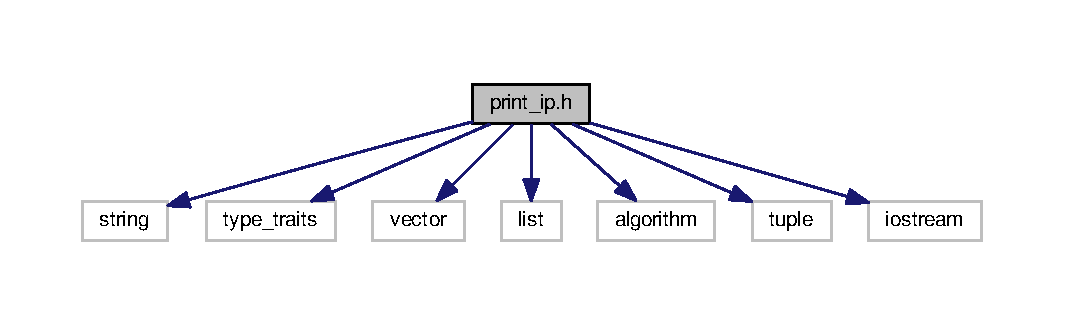
\includegraphics[width=350pt]{print__ip_8h__incl}
\end{center}
\end{figure}
This graph shows which files directly or indirectly include this file\-:
\nopagebreak
\begin{figure}[H]
\begin{center}
\leavevmode
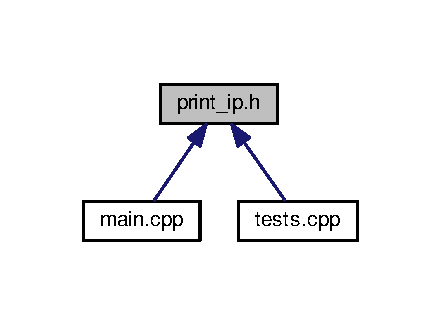
\includegraphics[width=211pt]{print__ip_8h__dep__incl}
\end{center}
\end{figure}
\subsection*{Classes}
\begin{DoxyCompactItemize}
\item 
class \hyperlink{classPRNT_1_1print__ip}{P\-R\-N\-T\-::print\-\_\-ip$<$ T, bool, bool $>$}
\item 
class \hyperlink{classPRNT_1_1print__ip_3_01std_1_1string_00_01false_00_01true_01_4}{P\-R\-N\-T\-::print\-\_\-ip$<$ std\-::string, false, true $>$}
\item 
class \hyperlink{classPRNT_1_1print__ip_3_01T_00_01false_00_01true_01_4}{P\-R\-N\-T\-::print\-\_\-ip$<$ T, false, true $>$}
\item 
class \hyperlink{classPRNT_1_1print__ip_3_01T_00_01true_00_01false_01_4}{P\-R\-N\-T\-::print\-\_\-ip$<$ T, true, false $>$}
\end{DoxyCompactItemize}
\subsection*{Namespaces}
\begin{DoxyCompactItemize}
\item 
\hyperlink{namespacePRNT}{P\-R\-N\-T}
\end{DoxyCompactItemize}
\subsection*{Functions}
\begin{DoxyCompactItemize}
\item 
{\footnotesize template$<$size\-\_\-t I = 0, typename... Tp$>$ }\\std\-::enable\-\_\-if$<$ I==sizeof...(Tp), \\*
void $>$\-::type \hyperlink{namespacePRNT_a034dd46fbd618b4c1e2d8b4612b676ef}{P\-R\-N\-T\-::print} (const std\-::tuple$<$ Tp...$>$ \&t)
\end{DoxyCompactItemize}

\hypertarget{tests_8cpp}{\section{tests.\-cpp File Reference}
\label{tests_8cpp}\index{tests.\-cpp@{tests.\-cpp}}
}
{\ttfamily \#include $<$map$>$}\\*
{\ttfamily \#include $<$tuple$>$}\\*
{\ttfamily \#include $<$iostream$>$}\\*
{\ttfamily \#include $<$sstream$>$}\\*
{\ttfamily \#include \char`\"{}print\-\_\-ip.\-h\char`\"{}}\\*
{\ttfamily \#include $<$boost/test/unit\-\_\-test.\-hpp$>$}\\*
{\ttfamily \#include $<$boost/test/output\-\_\-test\-\_\-stream.\-hpp$>$}\\*
{\ttfamily \#include $<$boost/any.\-hpp$>$}\\*
Include dependency graph for tests.\-cpp\-:
\nopagebreak
\begin{figure}[H]
\begin{center}
\leavevmode
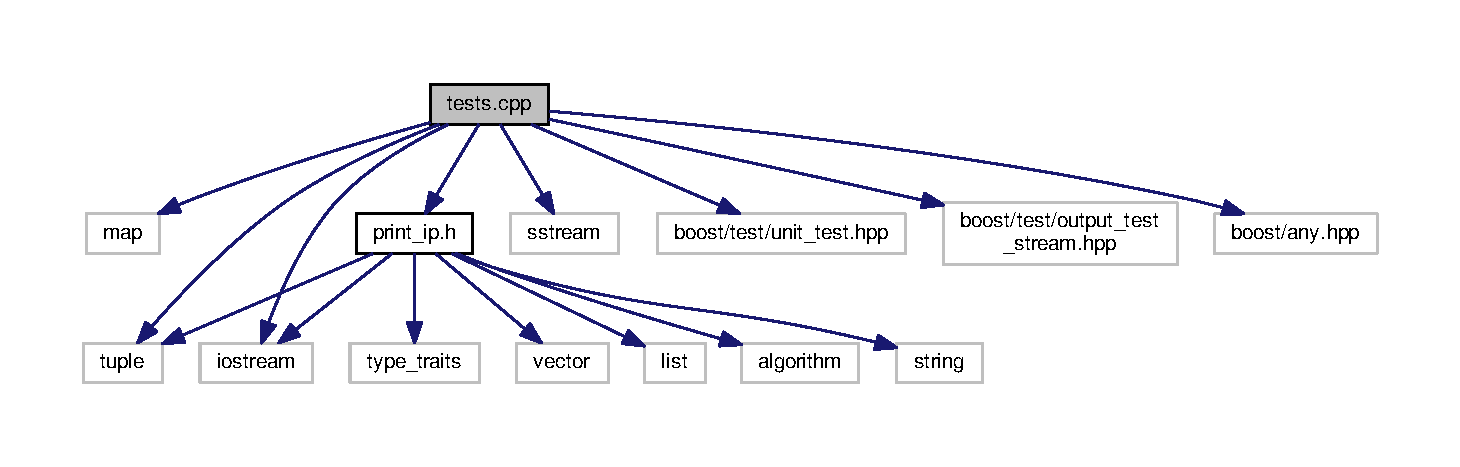
\includegraphics[width=350pt]{tests_8cpp__incl}
\end{center}
\end{figure}
\subsection*{Classes}
\begin{DoxyCompactItemize}
\item 
struct \hyperlink{structcout__redirect}{cout\-\_\-redirect}
\item 
struct \hyperlink{structhelper}{helper}
\end{DoxyCompactItemize}
\subsection*{Macros}
\begin{DoxyCompactItemize}
\item 
\#define \hyperlink{tests_8cpp_ab340a5e76af466a5f20ec5500d30a80b}{B\-O\-O\-S\-T\-\_\-\-T\-E\-S\-T\-\_\-\-M\-A\-I\-N}
\item 
\#define \hyperlink{tests_8cpp_a139f00d2466d591f60b8d6a73c8273f1}{B\-O\-O\-S\-T\-\_\-\-T\-E\-S\-T\-\_\-\-D\-Y\-N\-\_\-\-L\-I\-N\-K}
\item 
\#define \hyperlink{tests_8cpp_a6b2a3852db8bb19ab6909bac01859985}{B\-O\-O\-S\-T\-\_\-\-T\-E\-S\-T\-\_\-\-M\-O\-D\-U\-L\-E}~test\-\_\-main
\end{DoxyCompactItemize}
\subsection*{Typedefs}
\begin{DoxyCompactItemize}
\item 
using \hyperlink{tests_8cpp_a8790c352e0524c72b2c3a430e6b1d258}{any} = boost\-::any
\end{DoxyCompactItemize}
\subsection*{Functions}
\begin{DoxyCompactItemize}
\item 
{\footnotesize template$<$std\-::size\-\_\-t I = 0, typename Func\-T , typename... Tp$>$ }\\std\-::enable\-\_\-if$<$ I==sizeof...(Tp), \\*
void $>$\-::type \hyperlink{tests_8cpp_ac3e2c1e6e55705c61cb3552b93afae47}{for\-\_\-index} (int, std\-::tuple$<$ Tp...$>$ \&, Func\-T)
\end{DoxyCompactItemize}
\subsection*{Variables}
\begin{DoxyCompactItemize}
\item 
std\-::stringstream \hyperlink{tests_8cpp_a8fc3524f4e679a41dcc8d0f302d637ed}{ss}
\end{DoxyCompactItemize}


\subsection{Macro Definition Documentation}
\hypertarget{tests_8cpp_a139f00d2466d591f60b8d6a73c8273f1}{\index{tests.\-cpp@{tests.\-cpp}!B\-O\-O\-S\-T\-\_\-\-T\-E\-S\-T\-\_\-\-D\-Y\-N\-\_\-\-L\-I\-N\-K@{B\-O\-O\-S\-T\-\_\-\-T\-E\-S\-T\-\_\-\-D\-Y\-N\-\_\-\-L\-I\-N\-K}}
\index{B\-O\-O\-S\-T\-\_\-\-T\-E\-S\-T\-\_\-\-D\-Y\-N\-\_\-\-L\-I\-N\-K@{B\-O\-O\-S\-T\-\_\-\-T\-E\-S\-T\-\_\-\-D\-Y\-N\-\_\-\-L\-I\-N\-K}!tests.cpp@{tests.\-cpp}}
\subsubsection[{B\-O\-O\-S\-T\-\_\-\-T\-E\-S\-T\-\_\-\-D\-Y\-N\-\_\-\-L\-I\-N\-K}]{\setlength{\rightskip}{0pt plus 5cm}\#define B\-O\-O\-S\-T\-\_\-\-T\-E\-S\-T\-\_\-\-D\-Y\-N\-\_\-\-L\-I\-N\-K}}\label{tests_8cpp_a139f00d2466d591f60b8d6a73c8273f1}
\hypertarget{tests_8cpp_ab340a5e76af466a5f20ec5500d30a80b}{\index{tests.\-cpp@{tests.\-cpp}!B\-O\-O\-S\-T\-\_\-\-T\-E\-S\-T\-\_\-\-M\-A\-I\-N@{B\-O\-O\-S\-T\-\_\-\-T\-E\-S\-T\-\_\-\-M\-A\-I\-N}}
\index{B\-O\-O\-S\-T\-\_\-\-T\-E\-S\-T\-\_\-\-M\-A\-I\-N@{B\-O\-O\-S\-T\-\_\-\-T\-E\-S\-T\-\_\-\-M\-A\-I\-N}!tests.cpp@{tests.\-cpp}}
\subsubsection[{B\-O\-O\-S\-T\-\_\-\-T\-E\-S\-T\-\_\-\-M\-A\-I\-N}]{\setlength{\rightskip}{0pt plus 5cm}\#define B\-O\-O\-S\-T\-\_\-\-T\-E\-S\-T\-\_\-\-M\-A\-I\-N}}\label{tests_8cpp_ab340a5e76af466a5f20ec5500d30a80b}
\hypertarget{tests_8cpp_a6b2a3852db8bb19ab6909bac01859985}{\index{tests.\-cpp@{tests.\-cpp}!B\-O\-O\-S\-T\-\_\-\-T\-E\-S\-T\-\_\-\-M\-O\-D\-U\-L\-E@{B\-O\-O\-S\-T\-\_\-\-T\-E\-S\-T\-\_\-\-M\-O\-D\-U\-L\-E}}
\index{B\-O\-O\-S\-T\-\_\-\-T\-E\-S\-T\-\_\-\-M\-O\-D\-U\-L\-E@{B\-O\-O\-S\-T\-\_\-\-T\-E\-S\-T\-\_\-\-M\-O\-D\-U\-L\-E}!tests.cpp@{tests.\-cpp}}
\subsubsection[{B\-O\-O\-S\-T\-\_\-\-T\-E\-S\-T\-\_\-\-M\-O\-D\-U\-L\-E}]{\setlength{\rightskip}{0pt plus 5cm}\#define B\-O\-O\-S\-T\-\_\-\-T\-E\-S\-T\-\_\-\-M\-O\-D\-U\-L\-E~test\-\_\-main}}\label{tests_8cpp_a6b2a3852db8bb19ab6909bac01859985}


\subsection{Typedef Documentation}
\hypertarget{tests_8cpp_a8790c352e0524c72b2c3a430e6b1d258}{\index{tests.\-cpp@{tests.\-cpp}!any@{any}}
\index{any@{any}!tests.cpp@{tests.\-cpp}}
\subsubsection[{any}]{\setlength{\rightskip}{0pt plus 5cm}using {\bf any} =  boost\-::any}}\label{tests_8cpp_a8790c352e0524c72b2c3a430e6b1d258}


\subsection{Function Documentation}
\hypertarget{tests_8cpp_ac3e2c1e6e55705c61cb3552b93afae47}{\index{tests.\-cpp@{tests.\-cpp}!for\-\_\-index@{for\-\_\-index}}
\index{for\-\_\-index@{for\-\_\-index}!tests.cpp@{tests.\-cpp}}
\subsubsection[{for\-\_\-index}]{\setlength{\rightskip}{0pt plus 5cm}template$<$std\-::size\-\_\-t I = 0, typename Func\-T , typename... Tp$>$ std\-::enable\-\_\-if$<$I == sizeof...(Tp), void$>$\-::type for\-\_\-index (
\begin{DoxyParamCaption}
\item[{int}]{, }
\item[{std\-::tuple$<$ Tp...$>$ \&}]{, }
\item[{Func\-T}]{}
\end{DoxyParamCaption}
)\hspace{0.3cm}{\ttfamily [inline]}}}\label{tests_8cpp_ac3e2c1e6e55705c61cb3552b93afae47}


\subsection{Variable Documentation}
\hypertarget{tests_8cpp_a8fc3524f4e679a41dcc8d0f302d637ed}{\index{tests.\-cpp@{tests.\-cpp}!ss@{ss}}
\index{ss@{ss}!tests.cpp@{tests.\-cpp}}
\subsubsection[{ss}]{\setlength{\rightskip}{0pt plus 5cm}std\-::stringstream ss}}\label{tests_8cpp_a8fc3524f4e679a41dcc8d0f302d637ed}

\hypertarget{version_8h}{\section{version.\-h File Reference}
\label{version_8h}\index{version.\-h@{version.\-h}}
}
\subsection*{Macros}
\begin{DoxyCompactItemize}
\item 
\#define \hyperlink{version_8h_a4a5fc96a4bdd7d68ed99ccce9ca2e77e}{P\-R\-O\-J\-E\-C\-T\-\_\-\-V\-E\-R\-S\-I\-O\-N\-\_\-\-P\-A\-T\-C\-H}~18
\end{DoxyCompactItemize}


\subsection{Macro Definition Documentation}
\hypertarget{version_8h_a4a5fc96a4bdd7d68ed99ccce9ca2e77e}{\index{version.\-h@{version.\-h}!P\-R\-O\-J\-E\-C\-T\-\_\-\-V\-E\-R\-S\-I\-O\-N\-\_\-\-P\-A\-T\-C\-H@{P\-R\-O\-J\-E\-C\-T\-\_\-\-V\-E\-R\-S\-I\-O\-N\-\_\-\-P\-A\-T\-C\-H}}
\index{P\-R\-O\-J\-E\-C\-T\-\_\-\-V\-E\-R\-S\-I\-O\-N\-\_\-\-P\-A\-T\-C\-H@{P\-R\-O\-J\-E\-C\-T\-\_\-\-V\-E\-R\-S\-I\-O\-N\-\_\-\-P\-A\-T\-C\-H}!version.h@{version.\-h}}
\subsubsection[{P\-R\-O\-J\-E\-C\-T\-\_\-\-V\-E\-R\-S\-I\-O\-N\-\_\-\-P\-A\-T\-C\-H}]{\setlength{\rightskip}{0pt plus 5cm}\#define P\-R\-O\-J\-E\-C\-T\-\_\-\-V\-E\-R\-S\-I\-O\-N\-\_\-\-P\-A\-T\-C\-H~18}}\label{version_8h_a4a5fc96a4bdd7d68ed99ccce9ca2e77e}

%--- End generated contents ---

% Index
\newpage
\phantomsection
\addcontentsline{toc}{chapter}{Index}
\printindex

\end{document}
